\documentclass[11pt,a4paper]{article}

\usepackage[utf8]{inputenc}
\usepackage[T1]{fontenc}
\usepackage[spanish]{babel}

\usepackage{tgpagella}
\usepackage{geometry}
\usepackage{booktabs}
\usepackage{xcolor}
\usepackage{graphicx}
\usepackage{titlesec}
\usepackage{fancyhdr}
\usepackage[parfill]{parskip}
\usepackage[expansion=false]{microtype}
\usepackage{hyperref}
\usepackage{setspace}
\usepackage{needspace}
\usepackage{etoolbox}
\usepackage{ragged2e}

\widowpenalty=10000
\clubpenalty=10000
\displaywidowpenalty=10000

\hyphenpenalty=8000
\exhyphenpenalty=8000

\geometry{top=3.0cm,bottom=3.0cm,left=3.5cm,right=3.5cm}

\setlength{\parskip}{0.65em}
\setlength{\parindent}{0em}

\definecolor{azulai}{RGB}{30,80,140}
\definecolor{doradoai}{RGB}{140,90,0}
\definecolor{grisai}{RGB}{70,70,70}

\AtBeginDocument{\justifying}

\titleformat{\section}
{\Large\bfseries\color{azulai}\justifying}
{}
{0em}
{}
[{\color{azulai}\titlerule[0.5pt]}]

\titlespacing*{\section}
{0pt}{1.3em}{0.5em}

\titleformat{\subsection}
{\large\bfseries\color{doradoai}\justifying}
{}
{0em}
{}

\titlespacing*{\subsection}
{0pt}{1.0em}{0.35em}

\titleformat{\subsubsection}
{\normalsize\bfseries\color{grisai}\justifying}
{}
{0em}
{}

\titlespacing*{\subsubsection}
{0pt}{0.8em}{0.25em}

\preto\section{\Needspace{8\baselineskip}}
\preto\subsection{\Needspace{6\baselineskip}}
\preto\subsubsection{\Needspace{4\baselineskip}}

\pagestyle{fancy}
\fancyhf{}

\rhead{\textcolor{grisai}{\small Raquel Pain — Arquitectura Interna}}
\lhead{\textcolor{grisai}{\small Mercurio · Venus · Marte}}
\cfoot{\textcolor{grisai}{\small\thepage}}

\renewcommand{\headrulewidth}{0.3pt}

\hypersetup{
colorlinks=true,
linkcolor=azulai,
urlcolor=azulai
}

\setstretch{1.32}

\tolerance=1500
\emergencystretch=4em

\begin{document}

% ── Portada ──────────────────────────────────────────────────────────────────

\begin{titlepage}
  \centering

  \vspace*{2cm}

  {\Huge\bfseries\color{azulai} Mercurio · Venus · Marte}\\[0.6cm]

  {\large\color{grisai} Arquitectura Interna}\\[0.4cm]

  {\small\itshape\color{grisai}
  Procesamiento, vínculo y acción en el funcionamiento cotidiano
  }\\[2.2cm]

  {\huge\color{doradoai} Raquel Pain}\\[1.6cm]

  {\Large 07/05/1985 \quad 18:20}\\[0.35cm]

  {\Large Pamplona, España}\\[0.35cm]

  {\normalsize
  Lat: 42.8157° \quad
  Lon: -1.6522° \quad
  UTC+02:00
  }\\[0.35cm]

  {\normalsize
  Ascendente: Libra 14°36'
  \quad
  MC: Cáncer 17°21'
  }\\[2.2cm]

  \renewcommand{\arraystretch}{1.35}

  \begin{tabular}{ll}
    \textbf{Mercurio:} & Aries — Casa 7 21°12' \\
    \textbf{Venus:}    & Aries — Casa 6 8°52' \\
    \textbf{Marte:}    & Géminis — Casa 8 7°49' \\
  \end{tabular}

  \vfill

  {\small\color{grisai}
  Generado el 20/05/2026
  }

\end{titlepage}

\justifying

\tableofcontents

\clearpage

% ── Datos de referencia ───────────────────────────────────────────────────────
\section{Datos de referencia}

\begin{center}
\renewcommand{\arraystretch}{1.25}
\begin{tabular}{llll}
  \toprule
  \textbf{Planeta} & \textbf{Signo} & \textbf{Casa} & \textbf{Posición} \\
  \midrule
  Mercurio  & Aries  & 7  & 21°12' \\
  Venus    & Aries & 6 & 8°52' \\
  Marte    & Géminis & 8 & 7°49' \\
  Ascendente          & Libra           & ---                    & 14°36' \\
  Medio Cielo         & Cáncer            & ---                    & 17°21' \\
  \bottomrule
\end{tabular}
\end{center}
\justifying

\vspace{0.5cm}

\textbf{Aspectos entre planetas personales:}

\begin{center}
\begin{tabular}{lllll}
  \toprule
  \textbf{Planeta 1} & \textbf{Asp.} & \textbf{Planeta 2} & \textbf{Tipo} & \textbf{Orbe} \\
  \midrule
  Venus & sex & Marte & Sextil & 1.1° \\
  \bottomrule
\end{tabular}
\end{center}

\justifying

\vspace{0.7cm}

\begin{center}
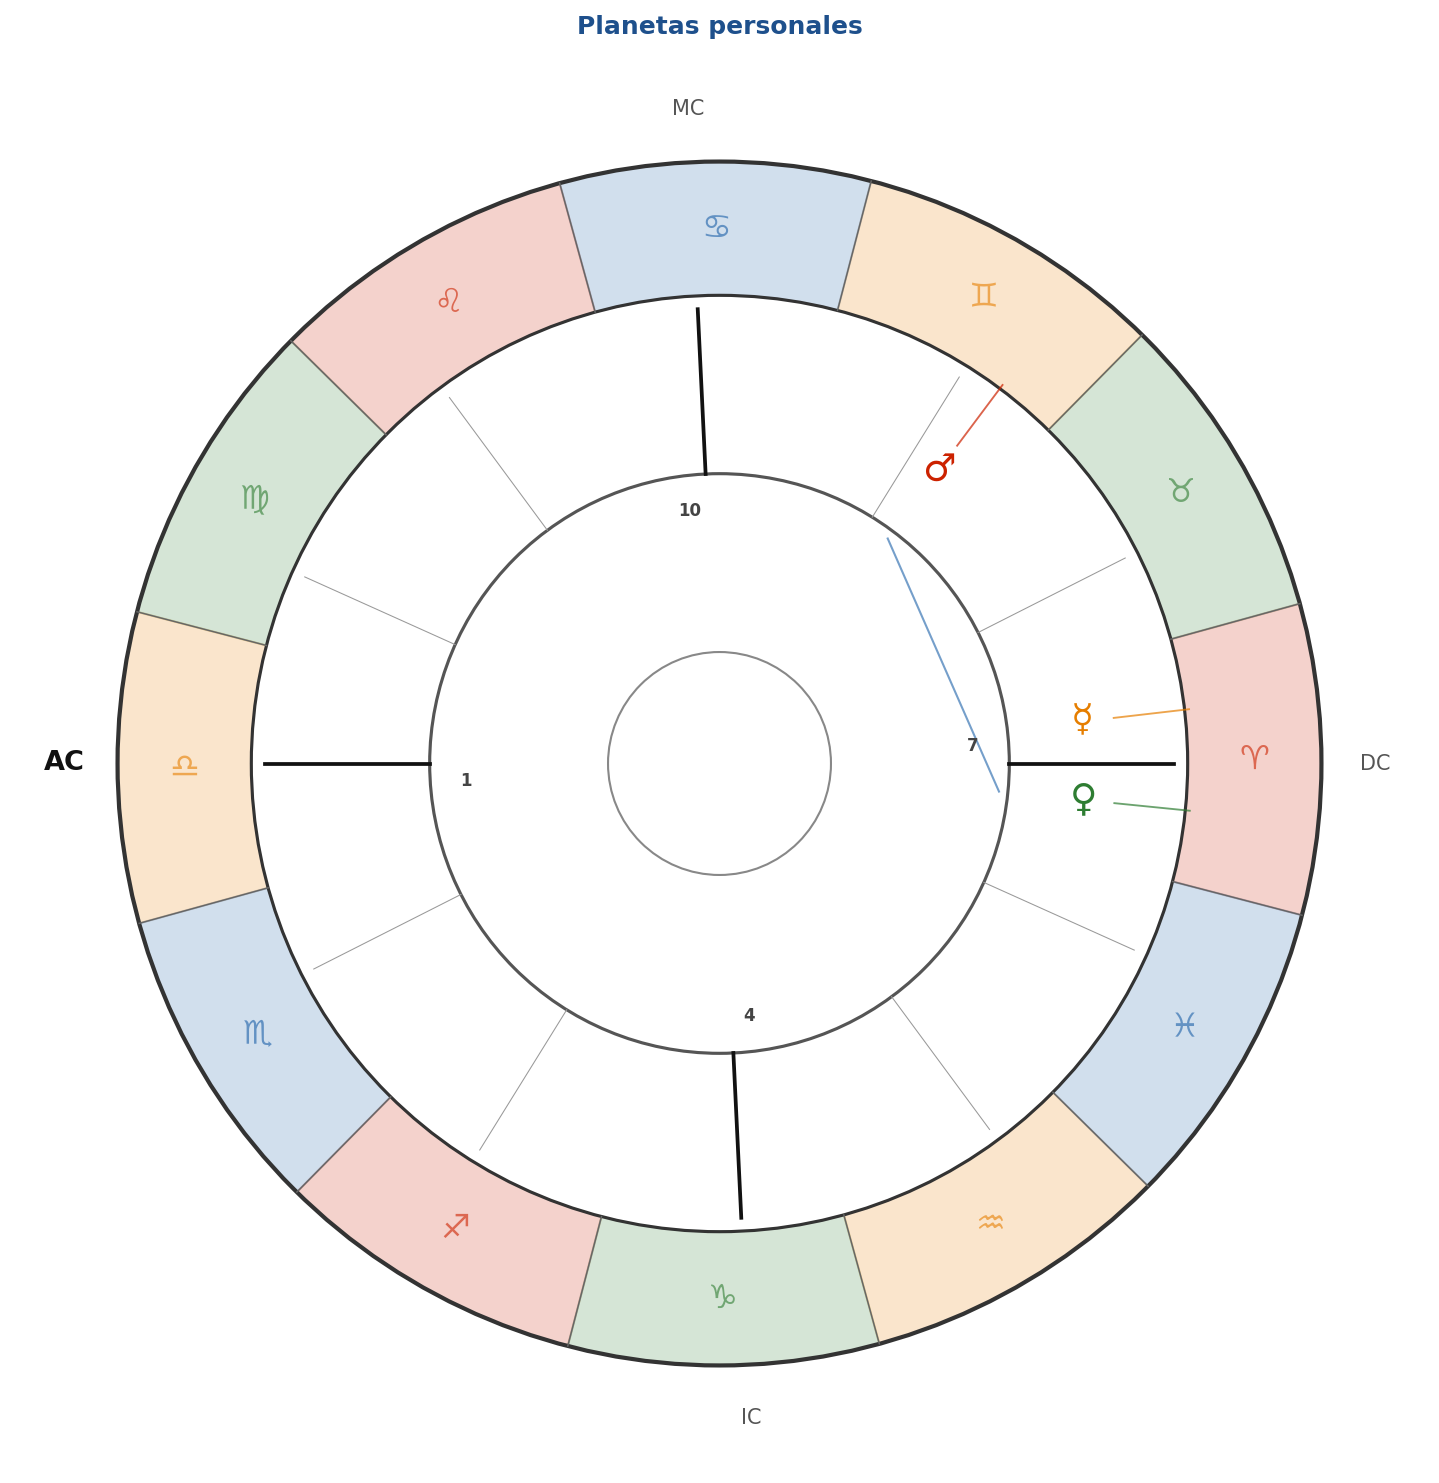
\includegraphics[width=0.72\textwidth]{Raquel_Pain_Planetas_Personales_rueda.png}
\end{center}

\vspace{0.3cm}
\Needspace{5\baselineskip}

% ── Interpretación ────────────────────────────────────────────────────────────
\section{Interpretación — Arquitectura Interna}

\begin{center}
{\small\itshape\color{grisai}
No se trata de describir la personalidad.\\
Se trata de observar cómo procesas, cómo te vinculas\\
y cómo se mueve tu energía en la vida cotidiana.
}
\end{center}

\justifying

\vspace{0.8cm}

% ── 1. Funcionamiento general ─────────────────────────────────────────────────
\subsection{1. Funcionamiento general}

\justifying
Mercurio está en Aries, Casa 7: muestra cómo piensas, cómo ordenas lo que percibes y cómo traduces lo que ocurre en palabras o ideas.
Venus está en Aries, Casa 6: muestra cómo te vinculas, qué necesitas para sentir conexión y cómo buscas equilibrio afectivo.
Marte está en Géminis, Casa 8: muestra cómo se activa tu acción, cómo descargas energía y cómo respondes ante el impulso.

Hay una concentración funcional entre Mercurio, Venus. Estas dos áreas tienden a activarse de forma cercana. Cuando una se mueve, la otra suele implicarse también. Esto puede dar fluidez, pero también puede hacer que cueste separarlas bajo presión.

Hay coherencia elemental entre: tu forma de pensar (Mercurio) y tu forma de vincularte (Venus) comparten elemento: Fuego; tu forma de pensar (Mercurio) y tu forma de actuar (Marte) se apoyan por elementos compatibles: Fuego/Aire; tu forma de vincularte (Venus) y tu forma de actuar (Marte) se apoyan por elementos compatibles: Fuego/Aire. Esto facilita que esas áreas colaboren entre sí. Aun así, lo que fluye con facilidad también puede volverse automático si no lo observas con consciencia.

Otros aspectos entre planetas personales: Venus–Marte en sextil (orbe 1.05°).

\vspace{0.8cm}

% ── 2. Mercurio ───────────────────────────────────────────────────────────────
\subsection{2. Mercurio — Pensamiento y procesamiento}

\subsubsection*{Mercurio en Aries — Casa 7}

\justifying
Tu mente funciona rápido y tiende a llegar a una conclusión antes de haber revisado todo el proceso. Sueles responder primero y comprobar después. Esto aporta rapidez real, capacidad de reacción y facilidad para decidir en movimiento.

La saturación aparece cuando hay demasiada información sin una prioridad clara. Si todo parece urgente al mismo tiempo, la velocidad se convierte en impaciencia y puedes actuar antes de haber terminado de entender. El bloqueo suele aparecer cuando hay que esperar, repetir algo varias veces o explicar en detalle algo que internamente ya sentías resuelto.

Sueles pensar mejor cuando puedes avanzar por pasos cortos, tomar decisiones concretas y descargar mentalmente la información mediante acción.

Necesitas diálogo para aclarar lo que piensas. Muchas veces entiendes mejor tus propias ideas cuando puedes contrastarlas con otra persona. El intercambio te ayuda a ordenar el pensamiento y ganar perspectiva.

La saturación aparece cuando dependes demasiado de la respuesta externa o cuando te cuesta sostener una posición propia sin validación. También cuando conversaciones importantes quedan abiertas durante demasiado tiempo. Sueles regularte mejor mediante diálogo claro, escucha mutua y espacios de intercambio equilibrado.

\vspace{0.8cm}

% ── 3. Venus ──────────────────────────────────────────────────────────────────
\subsection{3. Venus — Vínculo y regulación relacional}

\subsubsection*{Venus en Aries — Casa 6}

\justifying
Necesitas movimiento, iniciativa y espacio propio para sentirte bien dentro de una relación. La conexión suele funcionar mejor cuando puedes acercarte al otro sin sentir que pierdes autonomía.

La saturación aparece cuando la relación exige demasiada adaptación sostenida, espera constante o sensación de limitación. Entonces la energía afectiva disminuye rápidamente y aparece irritación o distancia. Cuando el vínculo deja de sostenerse, tiendes a tomar distancia antes de quedarte atrapade en algo que ya no se siente vivo.

Sueles regularte mejor en relaciones donde existe honestidad directa, espacio personal y sensación de movimiento compartido.

Necesitas cuidado concreto y presencia cotidiana para sostener el vínculo. Muchas veces expresas el afecto mediante pequeños actos, ayuda mutua y atención práctica a las necesidades de la otra persona.

La saturación aparece cuando la relación se convierte únicamente en responsabilidad o cuando el cuidado deja de ser recíproco. Entonces el vínculo empieza a sentirse más como obligación que como conexión real. Sueles regularte mejor mediante rutinas simples, cooperación y gestos cotidianos de cuidado mutuo.

En relación con los otros planetas personales:

Venus en sextil a Marte: existe compatibilidad entre vínculo y acción. Puedes relacionarte y actuar de forma complementaria cuando existe claridad y consciencia.

La conexión entre afecto y movimiento puede convertirse en un recurso importante tanto para relaciones como para proyectos personales.

\vspace{0.8cm}

% ── 4. Marte ──────────────────────────────────────────────────────────────────
\subsection{4. Marte — Acción y descarga}

\subsubsection*{Marte en Géminis — Casa 8}

\justifying
Tu energía se activa a través del pensamiento, la curiosidad y el intercambio mental. Necesitas movimiento cognitivo, variedad y estímulo para mantenerte en marcha. La acción descarga hablando, escribiendo, aprendiendo o cambiando de enfoque.

La saturación aparece cuando hay demasiados estímulos o demasiadas tareas abiertas al mismo tiempo. Entonces la energía se dispersa y cuesta terminar lo que empiezas. También puede aparecer inquietud verbal, aceleración mental o necesidad de discutir como forma de descarga.

Sueles regularte mejor mediante movimiento, conversación, escritura y actividades que permitan cambiar de foco sin perder dirección.

Necesitas profundidad e intensidad para sentirte plenamente activade. Tu energía descarga mejor en procesos transformadores, vínculos profundos o experiencias emocionalmente intensas.

La saturación aparece cuando la energía queda contenida durante demasiado tiempo o no encuentra espacios de descarga profunda. Entonces puede aparecer control excesivo, tensión interna constante o sensación de activación acumulada difícil de soltar. Sueles regularte mejor mediante intensidad consciente, honestidad emocional y procesos reales de transformación.

\vspace{0.8cm}

% ── 5. Integración ────────────────────────────────────────────────────────────
\subsection{5. Integración — Coherencias, fricciones y bucles}

\justifying
Hay una integración fuerte entre Mercurio, Venus. Estas áreas se activan de manera cercana y conviene observarlas juntas. A veces una de ellas expresa la tensión que en realidad empezó en la otra.

Mercurio y Venus comparten elemento en Fuego. Tu forma de pensar y tu forma de vincularte pueden comprenderse con relativa facilidad. Suele haber continuidad entre lo que percibes, lo que sientes y lo que necesitas expresar en relación.

Venus en sextil a Marte: existe compatibilidad entre vínculo y acción. Puedes relacionarte y actuar de forma complementaria cuando existe claridad y consciencia.

La conexión entre afecto y movimiento puede convertirse en un recurso importante tanto para relaciones como para proyectos personales.

Cuando hay demasiada presión, puede aparecer una cadena reconocible: Mercurio en Aries acelera hacia conclusiones antes de que el análisis esté completo. Desde ahí, Venus en Aries se aleja del vínculo o usa la relación como escenario de descarga. Y Marte en Géminis genera agitación que no siempre produce movimiento real. El ciclo se cierra cuando la energía acumulada vuelve a saturar el punto inicial.

\vspace{0.8cm}

% ── 6. Orientación práctica ───────────────────────────────────────────────────
\subsection{6. Orientación práctica}

\subsubsection*{Desde dónde empezar}

\justifying
Desde tu forma de pensar (Mercurio) en Aries, Casa 7. De las tres áreas, esta suele requerir menos energía para activarse. La entrada es activar el movimiento antes de intentar resolverlo todo mentalmente. Empezar por aquí puede abrir movimiento en el resto.

\subsubsection*{Qué sostener}

\justifying
Conviene sostener especialmente tu forma de actuar (Marte) en Géminis: espacio mental, palabra clara e intercambio regulado. Bajo presión, esta área puede desorganizarse antes que las demás. Cuando se estabiliza, el resto de tu funcionamiento tiene más capacidad para reorganizarse.

\subsubsection*{Qué evitar}

\justifying
Evitar asumir que la ausencia de fricción visible significa que todo está bien. A veces los bucles no hacen ruido porque te has acostumbrado a funcionar así.

\vspace{0.6cm}

\justifying
Si no se sostiene: pensamiento, vínculo y acción empiezan a funcionar por separado. Lo que piensas no alimenta la acción, la acción no informa al vínculo y el vínculo no regula la energía disponible. El esfuerzo aumenta, la claridad disminuye y la saturación llega antes.

\vspace{1.2cm}

\begin{center}
{\small\itshape\color{grisai}
La astrología se utiliza aquí como lenguaje simbólico de observación,\\
no como una definición cerrada de quién eres.\\[0.2cm]
Este documento propone una lectura funcional y orientativa, no un diagnóstico.
}
\end{center}

\end{document}
